\chapter{色表示、强子与禁闭}

\paragraph{一段简短的开场插曲。}
在回到群论之前，请允许我做一次不知羞耻的商业宣传。\emph{《黑洞战争》}讲述了与斯蒂芬·霍金之间关于黑洞是否会摧毁量子信息的漫长争论。它也记录了一些理论物理学家特有的残忍：不仅有薛定谔的猫，还有萨斯坎德的鱼以及它们不幸掉进马桶的遭遇。履行完这项义务后，我们回到爱丽丝和鲍勃。爱丽丝仍在受苦，因为鲍勃仍在逼她学习群论。

\lectureoverview{对称性通过它对态的作用而成为物理的。我们从转动开始，引入表示和生成元，然后对色\(SU(3)\)重复这一构造。色表示组合成强子，而它们的动力学解释了为什么从未观察到孤立的色。}

\section{群与它所作用的对象}

每一次关于对称性的讨论都包含两个观念。首先是一个抽象群：一组带有乘法法则、单位元和逆元的运算。其次是那些运算所作用的对象。这两个观念可以区分开来，但在物理学中它们无法分离。对称性之所以重要，是因为它变换物理态、场、坐标或可观测量。

\begin{classroomqa}
\audiencequestion{群既被描述为一张抽象的乘法表，又被描述为作用于物理对象的矩阵。这两个部分可以分离开来吗？
\lecturetimestamp{00:01:58}}
\lecturerresponse{它们是不同层次的描述，但完全相关。转动作为一种抽象运算存在，先于我们指定它转动什么。物理学随后追问，同一个运算如何作用于与特定系统相关的态和量。矩阵提供了这种具体的作}
\end{classroomqa}

空间转动提供了最清晰的例子。在经典情形下，同一个转动可以作用于粒子的坐标、磁体的方向，或任何其他矢量。在量子力学中，态生活在一个线性矢量空间中，因此转动由该空间上的一个线性算符表示。若\(g\)表示一个抽象群元素，而\(D(g)\)表示它的矩阵代表，则一致性意味着
\begin{equation}
D(g_1g_2)=D(g_1)D(g_2),
\qquad
D(e)=\boldsymbol 1.
\end{equation}
这些矩阵不必看起来像那些抽象运算，但它们的乘法必须重现群的乘法。
\editorialnote{同态方程明确写出了源文中口头描述的群乘法与矩阵乘法之间的对应关系。}

矩阵的维数由态空间决定，而不是仅由抽象群决定。如果我们只保留一个电子的自旋，那么有两种正交的可能性，自旋向上和自旋向下，而一个态是一个二分量的列矢量。因此转动通过\(2\times2\)矩阵作用。对于两个自旋二分之一的对象，有四个基态，
\begin{equation}
\ket{\uparrow\uparrow},\qquad
\ket{\uparrow\downarrow},\qquad
\ket{\downarrow\uparrow},\qquad
\ket{\downarrow\downarrow},
\end{equation}
而组合空间上的诱导作用是四维的。

熟悉的序列是
\begin{equation}
\begin{array}{c|c|c}
\text{spin} & \text{number of states} & \text{matrix dimension}\\
\hline
0 & 1 & 1\times1\\
\frac12 & 2 & 2\times2\\
1 & 3 & 3\times3\\
\frac32 & 4 & 4\times4
\end{array}
\end{equation}
依此类推。一个自旋为零的态给出平凡表示：每一个转动都让它保持不变。那个一乘一的矩阵就是\(1\)。一个自旋为一的态有三个分量，而它的转动矩阵就是熟悉的三维矢量转动。更一般地，自旋\(j\)有\(2j+1\)个态。

表示也可以是无限维的。如果我们描述一个电子的完整轨道运动，而不仅仅是它的自旋，那么一个态包含每一个位置的振幅，或等价地包含每一个动量的振幅。于是转动算符作用在一个无限维的波函数空间上。因此，同一个抽象转动群具有平凡的、二维的、三维的和无限维的表示。这正是当讨论从自旋转向色时我们将要复用的事实。

\section{为什么自旋转动是特殊酉的}

现在回到单个电子自旋，并舍弃它的轨道运动。转动由一个\(2\times2\)酉矩阵\(U\)表示，
\begin{equation}
U^\dagger U=\boldsymbol 1,
\qquad
U^{-1}=U^\dagger.
\label{eq:l4-unitarity}
\end{equation}
逆变换必须撤销该转动，而酉性保持范数，从而保持每一个概率。

一个一般的\(2\times2\)复矩阵包含四个复元素，即八个实参数。方程~\eqref{eq:l4-unitarity}施加四个独立的实条件，剩下四个参数。一个普通空间转动只有三个：两个参数选择轴，一个参数选择角。因此该酉矩阵多包含了一个相位。额外的限制是
\begin{equation}
\det U=1.
\label{eq:l4-det-one}
\end{equation}
于是计数为
\begin{equation}
8-4-1=3.
\end{equation}

行列式为一的限制在乘法下是稳定的，因为
\begin{equation}
\det(AB)=\det A\,\det B.
\end{equation}
如果两个矩阵的行列式都为一，那么它们的乘积的行列式也为一。它也与幺正性相容。对式~\eqref{eq:l4-unitarity}取行列式，得到
\begin{equation}
1=\det(U^\dagger U)
=\det(U^\dagger)\det U
=(\det U)^*\det U.
\end{equation}
因此，幺正矩阵的行列式位于单位圆上，
\begin{equation}
\det U=e^{i\phi}.
\end{equation}

\begin{classroomqa}
\audiencequestion{幺正性要求行列式为实数吗？
\lecturetimestamp{00:12:10}}
\lecturerresponse{不要求。幺正性只要求模为1。行列式可以是任意纯相位\(e^{i\phi}\)。对于二维矩阵，将\(U\)乘以\(e^{-i\phi/2}\)可以消去这个公共相位，得到一个行列式为1的矩阵。}
\end{classroomqa}

确实，如果
\begin{equation}
V=e^{-i\phi/2}U,
\end{equation}
那么\(V\)仍然是幺正的，并且
\begin{equation}
\det V=e^{-i\phi}\det U=1.
\end{equation}
行列式为1的幺正矩阵构成\(SU(2)\)。

有一个细微之处。人们很容易说\(SU(2)\)就是三维空间中的旋转群，但这一对应是二对一的。矩阵\(U\)和\(-U\)作用在旋量上不同，但它们对应普通矢量的同一个旋转。因此
\begin{equation}
SU(2)/\{\boldsymbol 1,-\boldsymbol 1\}\simeq SO(3).
\end{equation}
就目前的讨论而言，重要的是局部乘法结构和三个生成元，但双重覆盖解释了自旋二分之一的旋转的二值性。

\section{无穷小变换及其生成元}

有限旋转可以由许多非常小的旋转构建出来。接近单位元的群元素称为无穷小元素，而在连通群中，知道所有无穷小方向就足以通过反复乘法重构有限变换。对物理学而言更重要的是，生成这些无穷小变换的算符是与该对称性相关的守恒量。

将接近单位元的元素写为
\begin{equation}
U=\boldsymbol 1+i\epsilon T,
\qquad |\epsilon|\ll1.
\label{eq:l4-infinitesimal-u}
\end{equation}
因子\(i\)是一个方便的约定。代入幺正性并舍弃\(\epsilon^2\)阶的项，得到
\begin{align}
(\boldsymbol 1+i\epsilon T)
(\boldsymbol 1-i\epsilon T^\dagger)&=\boldsymbol 1,
\\
i\epsilon(T-T^\dagger)&=0,
\\
T&=T^\dagger.
\label{eq:l4-hermitian-generator}
\end{align}
生成元是厄米的，正如量子力学可观测量所必须的那样。

\begin{figure}[htbp]
\centering
\includegraphics[width=0.62\textwidth]{lecture_04_figure_03.png}
\caption{以\(T=T^\dagger\)结尾的接近单位元的幺正性计算。}
\lectureframe{00:23:28}
\end{figure}

对于空间旋转，有三个线性无关的生成元，因为有三个独立的无穷小轴。绕任意方向的小旋转由绕\(x\)、\(y\)和\(z\)的小旋转组合而成。相应的生成元是角动量算符\(J_x,J_y,J_z\)。它们的对易子编码了旋转的非对易性，
\begin{equation}
[J_i,J_j]=i\epsilon_{ijk}J_k.
\label{eq:l4-angular-momentum-algebra}
\end{equation}
反复的无穷小旋转随后构建出有限旋转。

我们已经使用了幺正性，但还没有使用行列式为1。对于任意小矩阵\(m\)，
\begin{equation}
\det(\boldsymbol 1+\epsilon m)
=1+\epsilon\,\operatorname{tr}m+O(\epsilon^2).
\label{eq:l4-det-expansion}
\end{equation}

\begin{figure}[htbp]
\centering
\includegraphics[width=0.62\textwidth]{lecture_04_figure_02.png}
\caption{黑板上开始写出的行列式一阶展开。}
\lectureframe{00:21:51}
\end{figure}

将式~\eqref{eq:l4-det-expansion}应用于
式~\eqref{eq:l4-infinitesimal-u}，
\begin{equation}
\det U
=1+i\epsilon\,\operatorname{tr}T+O(\epsilon^2).
\end{equation}
因此，特殊幺正条件要求
\begin{equation}
\operatorname{tr}T=0.
\label{eq:l4-traceless-generator}
\end{equation}
\(SU(2)\)的生成元正是无迹厄米
\(2\times2\)矩阵。该矢量空间的维数为三。一个标准基由泡利矩阵给出，
\begin{equation}
\begin{aligned}
\sigma_x&=
\begin{pmatrix}0&1\\1&0\end{pmatrix},
&
\sigma_y&=
\begin{pmatrix}0&-i\\i&0\end{pmatrix},
\\[0.4em]
\sigma_z&=
\begin{pmatrix}1&0\\0&-1\end{pmatrix}.
\end{aligned}
\end{equation}
对于自旋二分之一的表示，可以取\(J_i=\sigma_i/2\)，因此绕\(\hat{\boldsymbol n}\)转过角度\(\theta\)的有限旋转为
\begin{equation}
U(\hat{\boldsymbol n},\theta)
=\exp\!\left(-i\theta\,
\hat{\boldsymbol n}\cdot\boldsymbol\sigma/2\right).
\end{equation}
\editorialnote{有限指数是无穷小生成元讨论的标准完成。原文强调反复的小旋转，而不是明确写出这个公式。}

\begin{classroomqa}
\audiencequestion{所以有三个独立的无迹厄米\(2\times2\)矩阵？
\lecturetimestamp{00:24:07}}
\lecturerresponse{是的。它们就是三个泡利矩阵。对于\(3\times3\)特殊幺正矩阵，相应的数目是八，一个常规基由八个盖尔曼矩阵给出。}
\end{classroomqa}

\begin{classroomqa}
\audiencequestion{这个八与八重法和八种胶子中的``八''是同一个吗？
\lecturetimestamp{00:24:43}}
\lecturerresponse{数学上是同一种\(SU(3)\)表示论，但必须指明作用的是哪一种\(SU(3)\)对称性。历史上的八重法味对称性不是色\(SU(3)\)。八种胶子属于色\(SU(3)\)的伴随表示。}
\end{classroomqa}

\section{从SU(2)到色SU(3)}

现在把矩阵从\(2\times2\)增大到\(3\times3\)。一个一般的复\(3\times3\)矩阵有九个复矩阵元，因而有十八个实参数。条件\(U^\dagger U=\boldsymbol 1\)给出九个实约束，而\(\det U=1\)又去掉一个。因此
\begin{equation}
18-9-1=8.
\end{equation}
有八个独立的无穷小方向和八个无迹厄米生成元。与\(SU(2)\)不同，这个群不是普通三维空间的旋转群。它是作用在色上的内部对称性。

在把这些表示赋予夸克之前，先回顾复合表示是如何产生的。把两个自旋为二分之一的系统放在一起，并忽略它们的轨道运动。共有四个乘积态，但一次旋转并不会把四个态不可约地混合起来。三个组合按自旋一变换，
\begin{align}
\ket{1,1}&=\ket{\uparrow\uparrow},\\
\ket{1,0}&=\frac{1}{\sqrt2}
(\ket{\uparrow\downarrow}+\ket{\downarrow\uparrow}),\\
\ket{1,-1}&=\ket{\downarrow\downarrow},
\end{align}
而第四个按自旋零变换，
\begin{equation}
\ket{0,0}=\frac{1}{\sqrt2}
(\ket{\uparrow\downarrow}-\ket{\downarrow\uparrow}).
\end{equation}
因此
\begin{equation}
\boldsymbol 2\otimes\boldsymbol 2
=\boldsymbol 3\oplus\boldsymbol 1.
\label{eq:l4-two-spin-decomposition}
\end{equation}
对齐的态给出三重态的\(m=\pm1\)个成员，对称的零投影态补全它，而反对称组合则是单态。这就是角动量相加以及组合色表示背后的一般逻辑。

每当两个自旋为二分之一的自由度耦合时，都会出现同样的单态--三重态区分。在原子氢中，电子和质子的自旋形成超精细单态和三重态。正氢和仲氢对\(H_2\)分子中两个质子的核自旋使用同样的表示论。
\editorialnote{原文在指氢原子中的质子--电子自旋时使用了``正氢和仲氢''。数学分解是正确的；这里为了精确而区分了分子和原子名称。}

\subsection{三重态与反三重态}

单个夸克有三个色振幅。在选定的基下写出
\begin{equation}
q=
\begin{pmatrix}
q_r\\q_g\\q_b
\end{pmatrix},
\qquad
q'=Uq,
\qquad U\in SU(3).
\label{eq:l4-quark-triplet}
\end{equation}
这三个分量可以是一个夸克的状态振幅，也可以是产生红、绿、蓝夸克的三个场算符。群混合这三个分量。一个最初为红色的态，在色变换后一般会变成红、绿、蓝的叠加。这个基本的三维表示称为\(\boldsymbol 3\)。

对于反夸克，群通过夸克表示的复共轭作用。对式~\eqref{eq:l4-quark-triplet}取复共轭得到
\begin{equation}
\bar q'=U^*\bar q.
\end{equation}
这个表示记作\(\bar{\boldsymbol 3}\)。与\(U(1)\)的类比是直接的：如果电子场获得\(e^{i\theta}\)，那么正电子场获得\(e^{-i\theta}\)。夸克和反夸克的色变换正是这种共轭配对在非阿贝尔情形下的版本。

在恒等元附近，如果
\begin{equation}
U=\boldsymbol 1+i\epsilon T,
\end{equation}
那么
\begin{equation}
U^*=\boldsymbol 1-i\epsilon T^*.
\end{equation}
因此反三重态的生成元是\(-T^*\)，即符号相反的共轭。这正是反夸克带相反色荷的精确含义。

\begin{classroomqa}
\audiencequestion{在\(SU(2)\)情形下，复共轭表示会怎样？
\lecturetimestamp{00:36:19}}
\lecturerresponse{\(SU(2)\)二重态是一个特例：在涉及反对称epsilon张量的一个固定基变换之后，它的复共轭等价于原来的二重态。对于\(SU(3)\)，\(\boldsymbol 3\)和\(\bar{\boldsymbol 3}\)是真正不等价的表示。}
\end{classroomqa}
\editorialnote{对\(SU(2)\)基本表示在数学上精确的术语是赝实，而不是实。这一回应保留了原文所要表达的区分，同时纠正了术语。}

\section{组合色表示}

符号\(\otimes\)并不意味着把它旁边写出的数作普通乘法。它意味着两个态空间被组合起来。所得的张量积空间随后被重新组织成在群作用下彼此不混合的若干部分。

\subsection{两个夸克：\texorpdfstring{\(\boldsymbol 3\otimes\boldsymbol 3\)}{3 x 3}}

两个夸克有九个色基态：红--红、红--绿、红--蓝，以及其余六个有序对。把两个色指标组织成对称部分和反对称部分。对称部分有六个独立分量；反对称部分有三个。在\(SU(3)\)下，
\begin{equation}
\boldsymbol 3\otimes\boldsymbol 3
=\boldsymbol 6\oplus\bar{\boldsymbol 3}.
\label{eq:l4-three-times-three}
\end{equation}

\begin{figure}[htbp]
\centering
\includegraphics[width=0.68\textwidth]{lecture_04_figure_04.png}
\caption{两个夸克的乘积分解为一个反三重态和一个六重态。}
\lectureframe{00:39:33}
\end{figure}

反三重态可以通过用不变epsilon张量缩并两个夸克指标来显式表示，
\begin{equation}
(qq)^k_{\bar 3}
=\frac{1}{\sqrt2}\epsilon^{kij}q_iq_j.
\end{equation}
这个对象有三个分量，并且像反夸克一样变换。六个对称组合构成六重态。这里并不是说两个夸克在动力学上变成一个反夸克；而是说它们色波函数的一个部分与反夸克具有相同的变换规律。

\subsection{一个夸克与一个反夸克：\texorpdfstring{\(\boldsymbol 3\otimes\bar{\boldsymbol 3}\)}{3 ⊗ 反-3}}

一个夸克--反夸克色态可以看作一个 \(3\times3\) 矩阵
\(M_i{}^j=q_i\bar q^j\)。每个这样的矩阵都唯一地分解为其迹与无迹部分，
\begin{equation}
M=\frac{\operatorname{tr}M}{3}\boldsymbol 1
+\left(M-\frac{\operatorname{tr}M}{3}\boldsymbol 1\right).
\end{equation}
迹是一个单一的不变成分，而无迹部分有八个成分。因此
\begin{equation}
\boldsymbol 3\otimes\bar{\boldsymbol 3}
=\boldsymbol 1\oplus\boldsymbol 8.
\label{eq:l4-three-times-threebar}
\end{equation}
在归一化意义下，单态为
\begin{equation}
\ket{1}_{q\bar q}
=\frac{1}{\sqrt3}
(\ket{r\bar r}+\ket{g\bar g}+\ket{b\bar b}).
\end{equation}
它不能旋转成任何其他东西，因为它是不可变的。另外八个线性组合则在它们自身之间混合。它们给出伴随表示，即八个生成元在其中变换的同一个表示。

\subsection{三个夸克}

将第三个夸克与式~\eqref{eq:l4-three-times-three}结合。反三重态分支给出
\begin{equation}
\bar{\boldsymbol 3}\otimes\boldsymbol 3
=\boldsymbol 1\oplus\boldsymbol 8,
\end{equation}
因此三夸克乘积包含一个单态。完整地写为，
\begin{equation}
\boldsymbol 3\otimes\boldsymbol 3\otimes\boldsymbol 3
=\boldsymbol 1\oplus\boldsymbol 8\oplus\boldsymbol 8
\oplus\boldsymbol{10}.
\label{eq:l4-three-quark-full}
\end{equation}
色单态是完全反对称的红--绿--蓝组合，
\begin{equation}
\ket{1}_{qqq}
=\frac{1}{\sqrt6}\epsilon^{ijk}\ket{q_iq_jq_k}.
\label{eq:l4-baryon-singlet}
\end{equation}
因为只要两个指标相同，\(\epsilon^{ijk}\) 就为零，所以每个非零项都包含一个红夸克、一个绿夸克和一个蓝夸克，并且在交换下符号交替。

\begin{classroomqa}
\audiencequestion{非单态组合只是不太可能出现，因此它们的概率可以被忽略吗？
\lecturetimestamp{00:46:02}}
\lecturerresponse{不。问题在于能量，而不是小概率。一个孤立的非单态会把色场带到任意大的距离，并且在禁闭区域中会需要无界能量。这一陈述背后的动力学将在下文展开。}
\end{classroomqa}

\subsection{胶子八重态}

胶子场像式~\eqref{eq:l4-three-times-threebar}中的八重态那样变换。就色而言，它带有一个三重态指标和一个反三重态指标，并去掉了单态迹。示意地，
\begin{equation}
q\sim\boldsymbol 3,
\qquad
\bar q\sim\bar{\boldsymbol 3},
\qquad
G\sim\boldsymbol 8.
\end{equation}
这些符号命名的是变换规律；粒子并不字面地等于整数三和八。

第九个夸克--反夸克色组合，即正比于单位矩阵的组合，是一个单态，并且不与八重态混合。因此省略它在数学上是一致的：一个 \(SU(3)\) 规范场是无迹的，并且有八个成分，而不是 \(U(3)\) 规范场的九个成分。

\begin{classroomqa}
\audiencequestion{为什么自然界省略了额外的单态胶子？
\lecturetimestamp{00:49:00}}
\lecturerresponse{直接的群论答案是，单态是一个独立的不变扇区，因此八重态在没有它的情况下也能自洽地封闭。选择 \(SU(3)\) 而不是 \(U(3)\) 的更深层理由不在这里推导；它是从 QCD 现象学推断出的规范结构的一部分。}
\end{classroomqa}

\section{作为强子的色单态}

强相互作用的自由、有限质量粒子是色单态。这并不使夸克或胶子变得不真实；它意味着它们不会作为孤立的渐近粒子出现。基本的单态构造模式是
\begin{equation}
qqq,
\qquad
q\bar q,
\qquad
GG\ \text{and higher gluonic products}.
\end{equation}
它们分别导致重子、介子和胶球。若干已经无色的对象的乘积当然仍然无色，因此可以由这些成分构造出更复杂的多强子态。

\begin{classroomqa}
\audiencequestion{三夸克单态和夸克--反夸克单态叫什么，胶子也能形成单态吗？
\lecturetimestamp{00:51:38}}
\lecturerresponse{三夸克单态是重子；夸克--反夸克单态是介子。胶子也能组合成色单态。最简单的这类强相互作用态称为胶球，并且可以有两个以上的胶子参与。}
\end{classroomqa}

三个自旋为二分之一的夸克总是组合成总自旋为半整数，尽管轨道角动量可以改变出现的是哪一个半整数。夸克--反夸克介子具有整数自旋。纯胶子胶球也具有整数自旋。

对于两个胶子，黑板上的第一个陈述只是一个计数，
\begin{equation}
8\times8=1+63.
\end{equation}
总共有六十四个色态；一个组合是单态，其余六十三个属于非单态扇区。

\begin{figure}[htbp]
\centering
\includegraphics[width=0.68\textwidth]{lecture_04_figure_05.png}
\caption{黑板上两胶子态计数：六十四个态中有一个单态。}
\lectureframe{00:53:44}
\end{figure}

完整的不可约分解是
\begin{equation}
\boldsymbol 8\otimes\boldsymbol 8
=\boldsymbol 1\oplus\boldsymbol 8_S\oplus\boldsymbol 8_A
\oplus\boldsymbol{10}\oplus\overline{\boldsymbol{10}}
\oplus\boldsymbol{27}.
\label{eq:l4-eight-times-eight}
\end{equation}
维数正确地相加：
\begin{equation}
1+8+8+10+10+27=64.
\end{equation}
这两个八重态是不同的不变子空间，一个在两个伴随因子的交换下对称，另一个反对称。单态是能够形成胶球态的两胶子色道。
\editorialnote{黑板上首先只给出 \(8\times8=1+63\)。随后的课堂交流给出了所列出的不可约维数；这里按照标准 \(SU(3)\) 记号恢复了横线和对称性标签。}

\subsection{为什么可观测电荷是整数}

夸克电荷有两种类型，
\begin{equation}
Q_{\mathrm{up\text{-}like}}=+\frac23,
\qquad
Q_{\mathrm{down\text{-}like}}=-\frac13.
\end{equation}
因此三个夸克的总电荷为整数：\(-1,0,+1,\text{ or }+2\)，
具体取决于其中有多少个是上型夸克。一个夸克和一个反夸克同样具有
电荷 \(0\) 或 \(\pm1\)。胶子不带电荷。因此，由观测到的夸克表示构建的基本色单态具有整数电荷，
尽管其组分携带分数电荷。

\begin{classroomqa}
\audiencequestion{奇异夸克的电荷是多少？
\lecturetimestamp{00:56:08}}
\lecturerresponse{它是下型夸克，因此其电荷为 \(-1/3\)。三个家族重复相同的电荷模式：\((u,d)\)、\((c,s)\) 和 \((t,b)\)，每对中的电荷分别为 \(+2/3\) 和 \(-1/3\)。}
\end{classroomqa}

对于这种粒子内容，色单态性和整数电荷密切相关，但它们并不是相同的数学陈述。整数性还利用了刚才写出的特定标准模型电荷赋值。

\begin{classroomqa}
\audiencequestion{色单态是纠缠态吗？它与贝尔实验中的纠缠对具有相同的意义吗？
\lecturetimestamp{00:56:58}}
\lecturerresponse{单态色波函数确实是纠缠的：它是相干叠加，而不是各自具有确定颜色的乘积。原则上其组分可以被分离，但禁闭使得这种分离代价越来越高，并最终产生新的强子。因此，尽管该态是纠缠的，它并不是进行贝尔式操作的便利系统。}
\end{classroomqa}

\section{张量积方程的含义}

此时，乘法表值得更具体的解释。
设 \(\psi_i\) 和 \(\phi_j\) 为产生两个自旋二分之一对象的算符；它们可以描述两种粒子，例如电子和质子，或者在包含适当统计性质时描述同一粒子的两个副本。
每个指标取两个值。四个乘积
\begin{equation}
\psi_\uparrow\phi_\uparrow,
\quad
\psi_\uparrow\phi_\downarrow,
\quad
\psi_\downarrow\phi_\uparrow,
\quad
\psi_\downarrow\phi_\downarrow
\end{equation}
张成张量积空间。

如果群元素在每个因子上作用为 \(U\)，则它在乘积上作用为 \(U\otimes U\)。在分量形式中，
\begin{equation}
\psi_i\phi_j
\longmapsto
U_i{}^kU_j{}^\ell\psi_k\phi_\ell.
\label{eq:l4-product-action}
\end{equation}
这是一个四维表示，但它是可约的。反对称组合
\begin{equation}
\frac{1}{\sqrt2}
(\psi_\uparrow\phi_\downarrow
-\psi_\downarrow\phi_\uparrow)
\end{equation}
映射到自身，而三个对称组合在彼此之间映射。在适应这些组合的基下，每个乘积表示矩阵都取块对角形式，
\begin{equation}
D_{2\otimes2}(g)
\sim
\begin{pmatrix}
1&0\\
0&D_3(g)
\end{pmatrix}.
\label{eq:l4-spin-block-diagonal}
\end{equation}

\begin{classroomqa}
\audiencequestion{诸如 \(\boldsymbol 3\otimes\boldsymbol 3=\bar{\boldsymbol 3}\oplus\boldsymbol 6\) 这样的方程表示什么运算？
\lecturetimestamp{00:57:51}}
\lecturerresponse{左侧构成复合态空间。群作用于两个因子，因此混合乘积基态。右侧说明基变换将这些态分离为不变集合：三个反对称组合按反三重态变换，六个对称组合按六重态变换。加号表示备选空间的直和，而不是普通的数值加法。}
\end{classroomqa}

\begin{classroomqa}
\audiencequestion{我们怎么知道九个态分裂为 \(3+6\)，或 \(1+8\)，而不是比如 \(2+7\)？
\lecturetimestamp{01:04:39}}
\lecturerresponse{仅靠维数计数无法决定分裂方式。必须知道 \(SU(3)\) 拥有哪些不可约表示，并构造不变子空间，例如通过对称化指标、反对称化指标，或将迹与无迹部分分离。完整分类需要更多群论；这里我们只使用夸克和胶子所需的表示。}
\end{classroomqa}

不变 epsilon 张量使单态构造变得透明。对于
\(SU(2)\)，
\begin{equation}
\epsilon_{ij}U^i{}_kU^j{}_\ell
=(\det U)\epsilon_{k\ell}
=\epsilon_{k\ell}.
\end{equation}
因此 \(\epsilon_{ij}\psi^i\phi^j\) 是不变的。对于 \(SU(3)\)，三指标版本给出
\begin{equation}
\epsilon_{ijk}U^i{}_aU^j{}_bU^k{}_c
=(\det U)\epsilon_{abc}
=\epsilon_{abc},
\end{equation}
这证明了方程~\eqref{eq:l4-baryon-singlet}中三夸克态的不变性。

\begin{classroomqa}
\audiencequestion{能否明确展示为什么单态不发生变换？
\lecturetimestamp{01:07:18}}
\lecturerresponse{可以。用完全反对称的 epsilon 张量缩并所有基本指标。在变换下，矩阵的乘积将 epsilon 乘以 \(\det U\)。对于特殊酉矩阵，该行列式为 1，因此缩并后的态保持不变。在 \(SU(2)\) 中，这证明了双自旋单态；在 \(SU(3)\) 中，它证明了红--绿--蓝三夸克单态。}
\end{classroomqa}

\begin{classroomqa}
\audiencequestion{两个胶子八重态的完整分解是什么？
\lecturetimestamp{01:09:24}}
\lecturerresponse{它是方程~\eqref{eq:l4-eight-times-eight}中的分解：一个单态、两个八重态、一个十重态、一个反十重态和一个二十七维表示。两个八重态指标恰好有一种色单态组合。}
\end{classroomqa}

\begin{classroomqa}
\audiencequestion{三个夸克对应的完整分解是什么？
\lecturetimestamp{01:11:51}}
\lecturerresponse{物理上本质的回答是，它包含一个单态。完成算术运算即得式~\eqref{eq:l4-three-quark-full}：一个单态、两个八重态和一个十重态，共\(1+8+8+10=27\)个态。\editorialnote{讲师在交流过程中不记得完整的\(3\otimes3\otimes3\)分解。标准补全在此明确给出，并在此标注，而非归因于口头回答。}}
\end{classroomqa}

同样的想法可推广到双胶子空间。在朴素乘积基中，
\(SU(3)\)通过\(64\times64\)矩阵作用。在适应不可约组分的基中，这些矩阵是块对角的，
\begin{equation}
\begin{aligned}
D_{8\otimes8}(g)
&\sim
\operatorname{diag}\bigl(
1,D_{8_S}(g),D_{8_A}(g),
\\
&\hspace{4.8em}
D_{10}(g),D_{\overline{10}}(g),D_{27}(g)
\bigr).
\end{aligned}
\end{equation}
没有任何块与其他块混合，尽管每个块内的态彼此混合。

\begin{classroomqa}
\audiencequestion{张量积分解是否只是换到一个基，使大的表示矩阵变成块对角？
\lecturetimestamp{01:12:02}}
\lecturerresponse{正是如此。对于两个自旋，四维矩阵变成一个一维单态块和一个三维三重态块。对于两个胶子，六十四维矩阵变成维度为\(1,8,8,10,10,\text{ and }27\)的块。每个块在任意群变换下都是封闭的。}
\end{classroomqa}

\begin{classroomqa}
\audiencequestion{完整张量积空间内那些封闭部分之一有名称吗？
\lecturetimestamp{01:14:55}}
\lecturerresponse{它是一个承载子表示的不变子空间。当它不能再分解时，它承载一个不可约表示，即irrep。完整张量积是这些不可约组分的直和。\editorialnote{原始材料在课堂上未给出所询问的术语。标准表示论术语在回答中给出。}}
\end{classroomqa}

\begin{classroomqa}
\audiencequestion{当非单态十重态和其他表示被称为不存在时，是否意味着它们应被完全忽略？
\lecturetimestamp{01:15:36}}
\lecturerresponse{它们是合法的色扇区，在中间计算中很重要，但它们不会在实验室中作为孤立的有限能量粒子出现。是禁闭，而非表示论的失败，阻止它们成为自由的渐近态。}
\end{classroomqa}

\section{从南部色荷思想到禁闭}

色荷思想早于QCD的最终表述。南部阳一郎在1960年代初就已理解，一个隐藏的三值量子数可以解决一个引人注目的问题：夸克带有分数电荷，却未观察到自由分数电荷粒子。如果物理态被迫为色单态，夸克就以如上所述整数电荷组合出现。剩下的问题是动力学问题：是什么迫使所有有限能量自由态成为单态？

从电磁类比开始。一个电荷与一个相反电荷相吸。将它们拉近会降低能量；将同号电荷推到一起则需要做功。场本身储存正的能量，
\begin{equation}
E_{\mathrm{field}}
=\frac12\int d^3x\,\boldsymbol E^2
\end{equation}
在简单静电单位中。净电荷会使场延伸到系统外部很远，而紧密束缚的中性对只有短程偶极场。因此，中和会从外部移除场能。

想象将电磁耦合极大地增大。净电荷的场能代价会变得如此之大，以至于低能物体将绝大多数为中性，而提取一个带电组分可能变得极其昂贵。南部将这一直觉转移到色荷：八种色荷是八种胶子场的源，因此巨大的色场能可能禁止孤立的非单态。

这一直觉基本上是正确的，但QCD包含一个决定性的新特征。光子不带电荷，而胶子带色荷。光子不是经典电磁场的源，麦克斯韦方程是线性的：两个电磁波叠加并相互穿过。胶子在色八重态中变换，因此胶子作为其他胶子的源并与之相互作用。甚至单个胶子场的不同部分也相互作用。因此，非阿贝尔规范场是非线性的。

\subsection{通量管与线性势}

在长距离下，胶子自相互作用阻止色通量像普通电偶极场那样扩散。通量被挤压成连接夸克与反夸克的管。长管的场强和横截面积近似固定，因此该管储存近似恒定的单位长度能量。若\(\sigma\)表示该弦张力，则
\begin{equation}
V(R)\simeq\sigma R+\text{constant}
\qquad (R\ \text{large}).
\label{eq:l4-linear-potential}
\end{equation}

\begin{figure}[htbp]
\centering
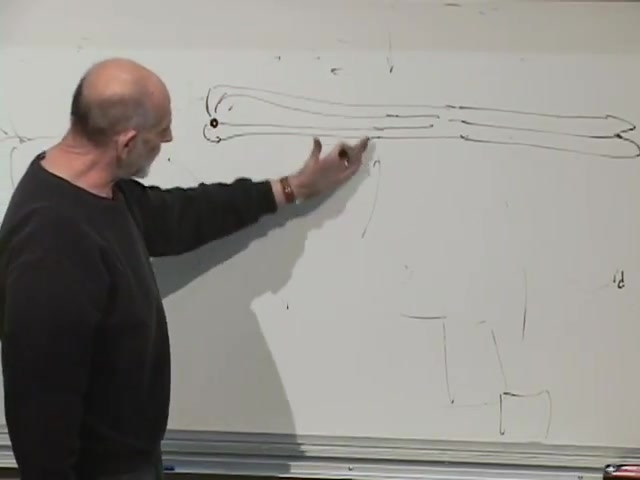
\includegraphics[width=0.78\textwidth]{lecture_04_figure_06.png}
\caption{色通量被束缚在夸克与反夸克之间的长管中。}
\lectureframe{01:31:35}
\end{figure}

这比库仑势更强，后者的量值按\(1/R\)下降。
把色源拉得更远并不会无限地削弱这个力；
它使管变长，并不断添加能量。在无限体积中，一个孤立的色荷将需要一根无限延伸的管，因此能量无界。这就是“只有色单态才具有有限能量的渐近态”这一说法的操作内容。
\editorialnote{弦张力记号与显式的长距离势，使源中关于均匀通量管每单位长度携带均匀能量的陈述定量化。}

\subsection{弦断裂与喷注}

假设一次硬碰撞击中介子内部的一个夸克。该夸克开始远离，但通量管在其后方被拉伸。它可能失去动能并被拉回。更常见的是，一旦储存的场能足够大，真空就会产生一对新的夸克--反夸克。新的反夸克终止了附着在逃逸夸克上的通量，而新的夸克终止了附着在原来反夸克上的通量。一个被拉伸的单态变成两个较短的\begin{equation}
(q\bar q)_{\mathrm{stretched}}
\longrightarrow
(q\bar q)+(q\bar q).
\label{eq:l4-string-breaking}
\end{equation}

\begin{figure}[htbp]
\centering
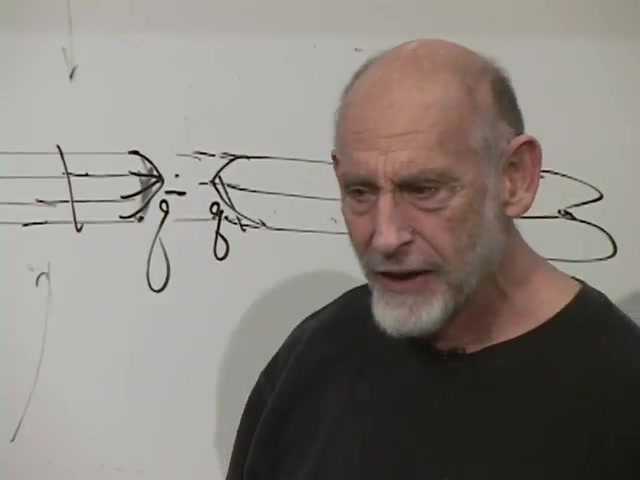
\includegraphics[width=0.78\textwidth]{lecture_04_figure_07.png}
\caption{对产生把一根被拉伸的通量管断裂成两根色单态管。}
\lectureframe{01:34:52}
\end{figure}

\begin{classroomqa}
\audiencequestion{如果一个被撞击的夸克具有足够的能量来持续拉伸这条管，那么除了它被拉回之外，还能发生什么？
\lecturetimestamp{01:33:50}}
\lecturerresponse{这条管可以通过夸克--反夸克对的产生而断裂。它的能量变成新产生的对的质量和动能。端点重新连接成两个单态，因此这一过程产生的是额外的介子，而不是一个孤立的夸克。}
\end{classroomqa}

如果这些部分子之一仍然携带大动量，该过程就会重复。结果是围绕原始部分子方向准直的一连串色单态强子：一个喷注。这种把高能夸克和胶子转化为强子的过程称为强子化。引发这一过程的带色客体是从喷注推断出来的，从未被单独观测到。

\begin{classroomqa}
\audiencequestion{弦断裂只产生介子，还是喷注中也能出现其他强子？\lecturetimestamp{01:35:20}}
\lecturerresponse{其他强子当然也能出现。唯一的颜色要求是最终可观测的客体必须是单态。介子是一次断裂的最简单图像，但重子、反重子以及更复杂的单态组合也可以产生。}
\end{classroomqa}

三个夸克可以在一个色单态结点处终止它们的通量。这个三分叉图像是方程~\eqref{eq:l4-baryon-singlet}中反对称epsilon张量的动力学对应物：没有净色通量从完整的重子中逃逸。

\begin{figure}[htbp]
\centering
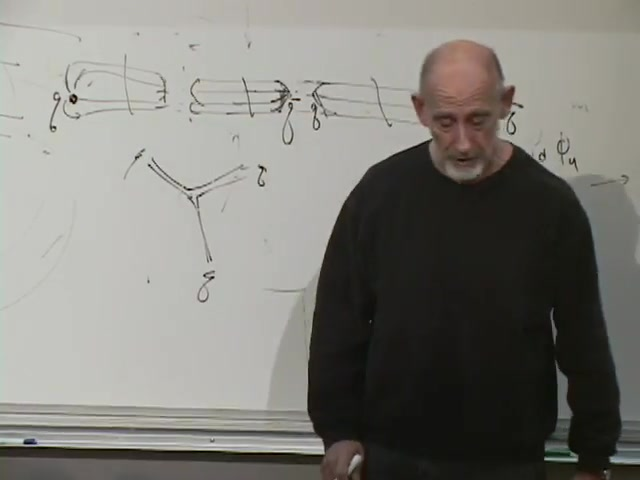
\includegraphics[width=0.72\textwidth]{lecture_04_figure_08.png}
\caption{重子的三分叉色通量结点，位于介子弦断裂示意图下方。}
\lectureframe{01:36:12}
\end{figure}

\section{规范场、守恒荷与标准模型}

在目前的层次上，规范理论可以被认为是一种理论，其中守恒荷作为光子类场的源。电荷是电磁场的源；八种色荷是八种胶子场的源。更深刻的表述使对称性成为局域的，并引入一个联络来比较相邻时空点上的内部态，但这里发展的禁闭图像并不需要那种构造。
\editorialnote{局域对称性表述是源中暗示但有意推迟的规范理论的标准更深层含义。}

对称性、守恒荷与通量紧密相连。如果场线只能终止于电荷上，那么一个源就不能简单地消失而其通量仍然附着于无物。它的全部远场也不能瞬时消失，因为场的变化以因果方式传播。在局域形式中，同样的物理由连续性方程表达，
\begin{equation}
\frac{\partial\rho}{\partial t}
+\boldsymbol\nabla\cdot\boldsymbol j=0,
\end{equation}
它表明电荷只能通过其边界流出才能离开一个区域。场线论证是这一局域守恒定律的几何图像。

现在我们可以把这一结果定位到标准模型之中。色贡献了\(SU(3)\)的八个生成元及其八个胶子场。阿贝尔部分提供一个生成元和一个规范场。另外三个生成元属于一个额外的\(SU(2)\)，而不是普通的空间角动量。在对称性破缺之前，规范结构为
\begin{equation}
SU(3)_c\times SU(2)_L\times U(1)_Y,
\end{equation}
共有\(8+3+1=12\)个生成元。接下来的任务是理解电弱\(SU(2)\)，然后是希格斯场，以及所观测到的光子、\(W^\pm\)和\(Z\)是如何出现的。
\editorialnote{该来源将光子与八个胶子归在一起，并把剩余因子描述为\(SU(2)\times U(1)\)。在未破缺的标准模型中，阿贝尔因子是超荷\(U(1)_Y\)；光子只有在电弱混合之后才出现。}

核心链条现在完整了。抽象群通过表示作用；无穷小生成元是守恒荷；夸克、反夸克和胶子分别占据\(\boldsymbol 3\)、\(\bar{\boldsymbol 3}\)和\(\boldsymbol 8\)；张量积识别出单态强子；而非线性胶子场把单态选择变成了禁闭这一物理现象。
